\chapter{Introduction}
\label{cha:Introduction}

\section{Motivation}
\label{sec:Motivation}
\subsection{Path planning in robotics}
In robotics the path planning of a robot can be programmed as a fixed list of movements to be executed. This has multiple drawbacks as for every change in the enviroment the robot needs to manually be reprogrammed.\\
But what if we equip this robot with a camera that detects the shape of objects in the robots enviroment. This would give us a set of objects at certain position, a robot arm in a starting position and a target where the robots endeffector needs to work. If we would be able to solve this puzzle, we could direct the robot in a different way each time without the actual need to access its software.


\subsection{Geometric riddles in gaming}
Solving geometric riddles is a amazingly fun task for a human. This is the reason many games simply consists of such riddles ranking from easy to hard in difficulty. But even the easiest riddle for a human proposes a big challenge for a simple algorithm that searches trough the possible ways of solving it. Even more complicated is the generation of such riddles. Even for the human brain this task can be exceedingly stressful.\\
 Now, if there would be a possibility to check if such a riddle has a solution, there would be the option to generate them randomly and check for feasability. This would release the developers of the need to manually create each riddle. Also the consumers, in this case the players, would have a never ending stream of new and different riddles to solve.

\section{State of the art}
\subsection{Pathplanning}
The correct answer to the question "Which algorithm is the best for finding the path from start to target" is not as easy as one might suspect. 
It depends on many factor including which structure one searches on ( e.g. graph, net, tree ), what knowledge there is about the current position ( e.g. distance to target ) and what result is needed ( shortest path, "good" path, existence of a path ).\\
For this work the focus is on a algorithm working on a graph with non-negativ edges, an absolute knowledge of the position of the target and the current in a two dimensional coordinate system and a need for a "good" path, not necessarily the shortest. Given these conditions, A$^\star$ is a valid choice. It is a widely used algorithm which calculates a "good" path, not a perfect one. How good the path is depends heavily on the heuristic used. In our case that would be a weighted sum of the distance traveled in steps plus the absolute distance to the target.\\
Another choice could be Dijkstra's algorithm \ref{ComputerScience} itself which is basically A$^\star$ with the heuristic set to constant zero. This would return the shortest path for all calculations. For the named applications from \ref{sec:Motivation} we need the algorithm to be fast more than to be precise thus A$^\star$ is the better choice.\\
It should be noted though that the algorithm for pathplanning is exchangable easily, as long as it is possible to create the graph while searching.

\subsection{Collision detection}
Collision detection in computer science has its home in simulations and computer games as it has in robotics. In this case the focus lies on the way computer games solve collision detection without looking into physical problems that would arise with it.\\
There are a number of ways this hase been solved. In a case where there are not that many objects needed to check, pairwise checking is an option. Depending on how the objects are represented, they need to be checked for collision for every step taken. A way around this is to bound objects, that lie in a certain proximity, together in spheres where they are only checked in paris if the objects spheres collide.\\
Also there is a difference it checking if a collision happened, or if it is about to happen. The first option is easy to calculate, because all that is needed is the current position of the objects concerned. The second needs to take into account the movement of all the objects that could collide. In this work, all algorithms know about the movement of the objects so the other option will be neglected.\\
Knowing about the movement allows to check only the objects lying in the way. To determine these obstacles two major algorithms are present.
One way is to start building a spacial binary tree starting from the object, partioning space along the direction of the movement. Until a given spacial size of an end node is reached ( e.g. the bounding box of the moving object) or a obstacle is in the node, the tree keeps on growing. The node directly in front of the last obstacle node would then be choosen as the last safe position to move to.\\
Another way is to build bounding boxes around all object and calculate a plane in space from the moving objects  and checked for collision with the bounding boxes by post-collision algorithms. This would give us the distance to the next obstacle in the moving direction, thus allowing us to stop our movement upon reaching it.\\
This last concept is used and refined to work with convex hulls for calculating the occuring collisions one of the implemented algorithms.


\subsection{Applications}
The standart solution in path planning for industrial robots is to hard-code the correct path. This is mostly done by setting a number of safe points on the path from start to target to avoid collision. \\
As a matter of fact, this is a good solution for processing objects where only one simple step for a large quantity is needed. In this scenario only few recalibrations are needed. But if the processed objects change more often, each time the machinist needs to recalibrate the robot. Using this algorithm instead, the objects can be treated as fixed obstacles holding the target. The endeffektor of the robot is the main object. Furthermore the robots links are movable obstacles whose movements depend on the movement of the endeffektor. \\
\newline
The automated creation of geometric riddles is a process widely used in the gaming industry. Not only riddles, whole characters and worlds are created at random.
One of the first famous games that made use of that was Nethack \ref{nethack}. It featured enemy characters and in closed randomized levels. This concept is still in use in todays products. The problem is, that this randomized content is created reverse. You would for example start with a valid riddle/ level, and then by doing only steps from a certain predetermined set of valid transformations reach a randomized mutation which can be used as new content.\\
The way one could create riddles with this algorithm is very different. There would be the option to place "totally" random objects into the riddle and afterwards check for the existence of a solution. "Totally" is put in  quotation marks is because there is still the need to look at the given properties of the riddle. For example if the riddles total space should only be 16x16 units big, putting an object the size of 1x30 units in would be not possible.

\section{Idea}
\label{sec:Idea}
As the representation behind these two cases is the same, for simplification purposes we break the riddles down into two dimensional object displacement problems. The following riddles shall provide simple example of the problem:\\

\begin{figure}[h]
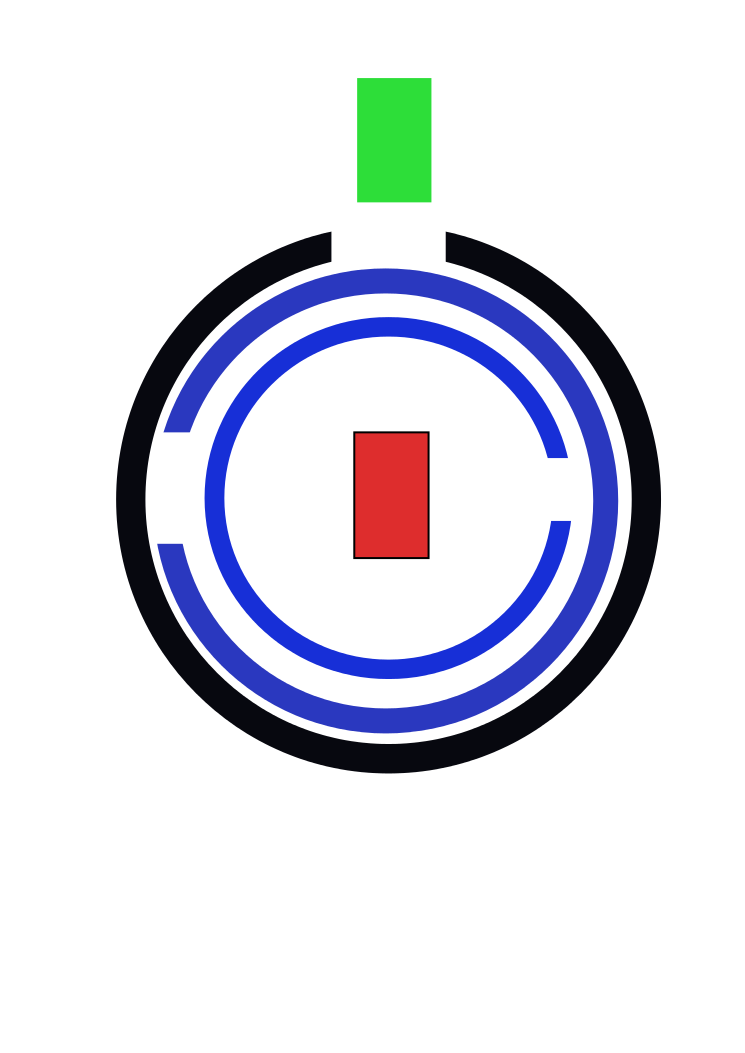
\includegraphics[scale=0.1]{circleRiddle.png}
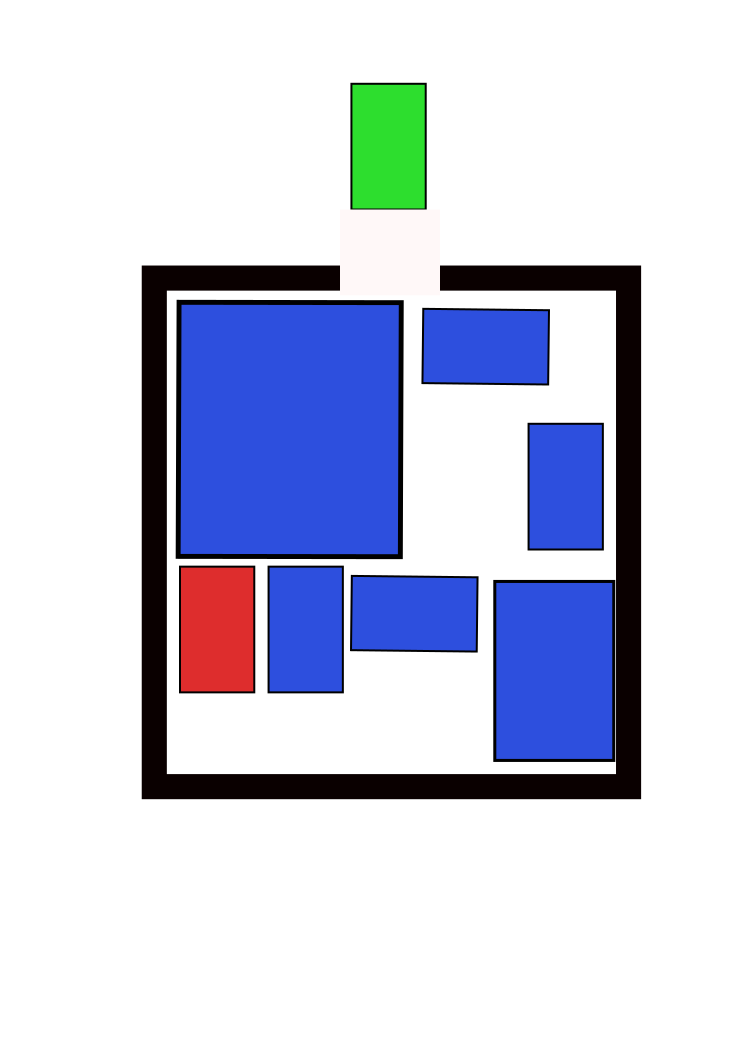
\includegraphics[scale=0.1]{boxRiddle.png}
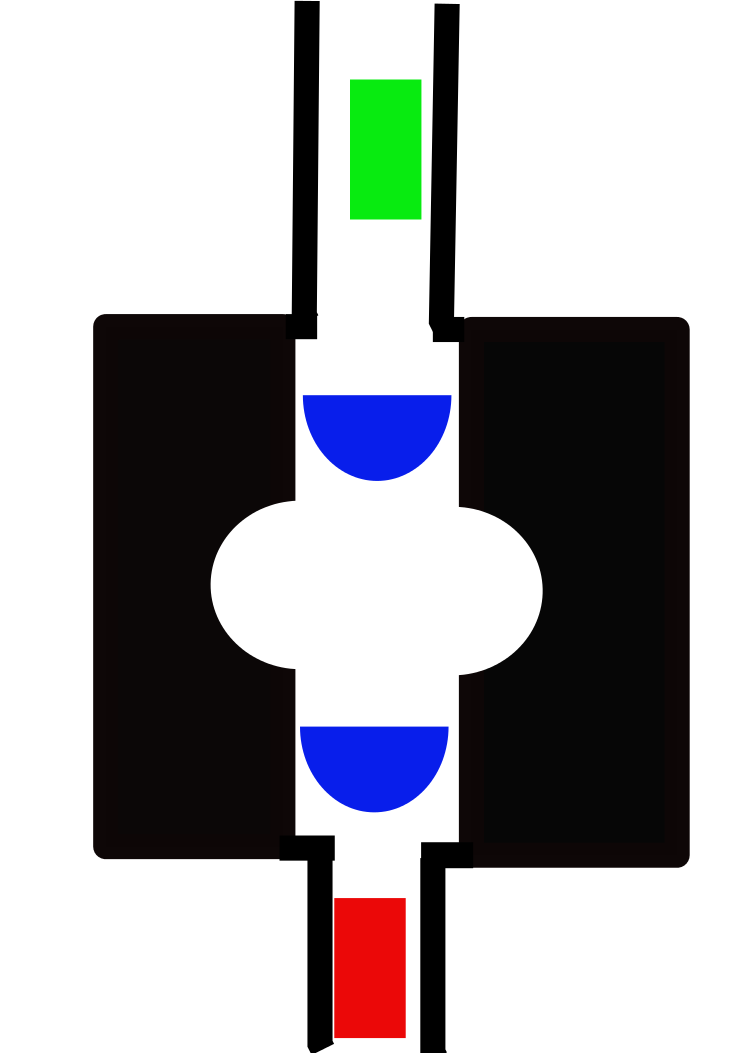
\includegraphics[scale=0.1]{mixedRiddle.png}
\caption{riddle 1 with circles , riddle 2 with boxes , riddle 3 with 2 half-circles}
\end{figure}

The riddle is solved, if the red box matches the green one. Blue objects are movable and black ones are stationary. The stationary ones will be referred to as rims hereafter.\\
As a human the way to solve those is quite obvious. The first riddle is solved by rotating the blue objects, the second through translation. The third needs both ways to be solved.\\
If we want to solve this with an algorithm, we would need to consider each objects collsision with the other objects and the rim. Also we would need to find a way to express the current configuration consisting of position (x,y) and rotation ($\phi$) and the direction the main object needs to take. A simple idea would be to 
\begin{enumerate}
\item generate all valid configurations per object in regard to the stationary obstacles as a configuration space
\item Create one collision space per object for collision with every other object. 
\item Substract the collision space from the configuration space to get valid space in regard to all obstacles for one object.
\item Divide the space in cells and locate the valid ones.
\item Build a graph out of this starting position by adapting the space after each step.
\item Search in that graph to get path from start to target point.
\end{enumerate}

The target point would then be a simple configuration vector holding each position of each object. A user defined distance function beetween start and target point in that space can then be used as heuristic in the graph search ( e.g. $h(start,target) = || ( x_{start} -  x_{target} , y_{start} - y_{target} ) ||$ ).
